\documentclass[11pt]{upenndiss}

\usepackage[all]{xypic}
%bibliography
\usepackage{natbib}
\bibpunct[:]{(}{)}{,}{a}{}{,}

% phonological examples

% fonts
\usepackage[normalem]{ulem}
\usepackage[T1]{fontenc}
%\usepackage{mathspec}
%\setmainfont[Mapping=tex-text]{Linux Libertine}
%\setmathfont(Digits,Greek,Latin){Linux Libertine}
%\usepackage{microtype}
%\usepackage{coptic}

\usepackage{setspace}

% tables and figures
\usepackage{booktabs}
\usepackage{floatrow}
\usepackage{enumitem}
\setlist{noitemsep}
\usepackage{multirow,sectsty}
\usepackage{subfigure,graphicx}

% Add packages and definitions you want to use here:
\usepackage[papersize={8.5 in, 11 in}, nohead, left=1.5 in, right = 1 in, vmargin= 1 in]{geometry}

%\usepackage{times}


%\usepackage{tipa}




% titles
\title{Parameterising Germanic ditransitive variation:\newline A historical-comparative study}
\author{Hezekiah Akiva Bacovcin}
\supervisor{Anthony Kroch}

\copyrighttrue
\department{Linguistics}

% Abstract
\abstractfile{Abstract} 
% Acknowledgement
\acknowledgementsfile{Acknowledgements}

% Dedication
%\dedication{
%}



\usepackage{gb4e}
\noautomath

\begin{document}

\thispagestyle{empty}\enlargethispage{\the\footskip}%
\null\vskip.1in%
\begin{center}
        {\setstretch{2.5} \MakeUppercase{Parameterising Germanic ditransitive variation}\par }%
        \vskip.3in
        Hezekiah Akiva Bacovcin
        \vskip .3in
        A DISSERTATION \\[.1in]
        in \\[.1in]
        Linguistics
        \vfill
Presented to the Faculties of the University of Pennsylvania in Partial \\
Fulfillment of the Requirements for the Degree of Doctor of Philosophy
\\[0.3in]
        2016
  \end{center}
  
  \parbox[t]{12cm}{\parindent=0pt Supervisor of Dissertation \vskip 0.5in
  \par \hrule width 7cm \vskip .1in Anthony Kroch, Professor of  Linguistics}
  
  \vskip 0.3in
  
  \parbox[t]{12cm}{\parindent=0pt Graduate Group Chairperson \vskip 0.5in
  \par \hrule width 7cm \vskip .1in Rolf Noyer, Associate Professor of Linguistics}

  \vskip 0.3in
  
  \parbox[t]{12cm}{\parindent=0pt Dissertation committee 
  \vskip -.1in
  David Embick, Professor of Linguistics
  \vskip -.1in
  William Haddican, Associate Professor of Linguistics, CUNY
  \vskip -.1in  
  Julie Legate, Professor of Linguistics
  \vskip -.1in
  Don Ringe, Professor of Linguistics
  }



\newpage 


\FrontMatter

% {\addcontentsline{toc}{chapter}{\listtablename}\listoftables}

%%%%%%%%%
%\chapter{Introduction}
\chapter{Introduction}
\label{ch:introduction}

% Larger picture situation
This dissertation addresses three larger questions: (a) what is the distribution of labour between the syntactic and morphological components of the grammar, (b) what aspects of syntax are universal/language particular, and (c) what methods can/should be used to address morphosyntactic problems. The first question bears on the architecture of the grammar, namely which surface properties are driven by the presence/absence/position of syntactic atoms and which properties are driven by the phonological (and semantic) realisation of those atoms. The answer to this question ideally reduces surface complexity to the interaction of simple independently necessary syntactic and morphological operations.

The second question (what aspects of syntax are universal/language particular) has direct implications for Plato's Problem, namely how do children acquire language as quickly as they do. Assuming that only language particular material needs to be acquired, the more universal properties that can be ascribed to human language, the easier it is to solve Plato's Problem \citep{Chomsky.1993}. The specific aspect of this question addressed here is the tension between argument structure and movement operations; different word orders could arise either by (a) being base generated in each position or (b) created by moving arguments from a previous (moved or base generated) position. This dissertation argues that there is no variation in base generation (the strong version of the UTAH hypothesis, \citealt{Baker.1988}) and that syntactic variation comes from differences in movement operations, morphological realisations, and associations of particular semantic concepts with the universally provided base constructions.

The answer to the final question (what methods are necessary to address morphosyntactic problems) depends on the nature of the problems being considered. The first question (on addressing the derivation of surface complexity) requires studying situations that involve some degree of surface complexity. However, in most cases, it is impossible to tease apart closely related solutions by looking at a single construction in a single language. The need to consider data from multiple sources is even more acute in the case of the second question. In order to plausibly argue for universality, it is necessary to demonstrate that the universal analysis has empirical coverage over a variety of distinct surface realisations. This dissertation solves this problem in two ways: (a) by using data from languages throughout the Germanic family and (b) bringing in qualitative and quantitative analysis of language change.

Typological study of closely related languages permits necessary comparisons. Often one language cannot provide the necessary data to support any given analysis (the crucial data is ambiguous or the necessary constructions do not exist for reasons irrelevant to the current theoretical question). However, a closely related language often provides the needed data, while being similar enough to the first language that we can be confident that the relevant theoretical implications are the same. The Germanic language family has the advantage of containing a number of well studied languages (including English, which has received the largest share of linguistic inquiry of any language), which provide a large amount of morphosyntactic variation (e.g., presence/absence of complex inflectional morphology and OV vs. VO word order). This variation, however, occurs within the framework of familial similarity that comes from all the languages being derived from a common ancestor. Variation within a broader framework of similarity helps reveal true comparisons between related elements, which might otherwise be obscured by irrelevant differences between the languages in question.

Another reason to study Germanic languages is the ability to do large scale quantitative diachronic research. Traditional syntactic inquiry has relied on the use of acceptability judgements to probe grammatical structure. However, it has been noted since the beginnings of the generative program that acceptability judgements are not a perfect probe for grammatical structure (see \citealt{Schutze.1996} for a discussion of the history of this issue). While acceptable sentences (when the judgement was given after long deliberation) are presumably all grammatical, ungrammaticality is only one of a number of factors that can contribute to unacceptability. Generative linguistics has developed a number of techniques for trying to overcome this issue (e.g., the use of multiple different lexicalisation and providing explicit contexts to alleviate pragmatic issues), quantitative corpus data provides an independent source of information about grammatical structure (\citealt{Kroch.1989,Kroch.1994} and others working in this programme). We can be more confident in conclusions that are supported by both sources of information (since they tap into different aspects of the grammatical processes and thus the probability that both would coincidently point to the same conclusion is much smaller than the probability that either would individually).

The case study that I have used to address the first two questions is the analysis of recipients in Germanic ditransitives. Ditransitive clauses provide the necessary surface complexity to be able to study how different grammatical components interact to produce that complexity. By constraining my focus to a particular semantic feature (recipients), I legitimate cross-linguistic comparisons in looking for universals. Assuming that all languages have the expressive capacity to capture any semantic notion and by  holding semantics constant, we can study  what morphosyntactic correlates of the semantics are universal and which are subject to linguistic variation.

The main theoretical claim of the dissertation is that recipients are universally base generated as dative PPs in the specifier of an applicative phrase (henceforth the dative PP + applicative analysis). As the dissertation progresses, a number of ancillary morphological and syntactic operations will be argued for to generate the surface complexity seen in Germanic. While none of the components (main or ancillary) are original, this dissertation provides a unique combination of previous theoretical proposals. Also, while cross-linguistic study of Germanic ditransitives have been employed previously (\citealt{Falk.1990}, \citealt{Sprouse.1995}, and \citealt{Holmberg.1995}, among others) this dissertation is the first complete survey of Germanic ditransitive data from all (major) extant Germanic languages. As such, all natural language examples are collected by language in an appendix for ease of reference.

The dissertation has the following structure. Chapter \ref{ch:theoryback} presents the theoretical background for the dissertation. This chapter focuses on presenting the theoretical claims in an abstract way independent from the inherent messiness of any natural language examples. Each component of the main claim is explicated. The focus is on the claims relevant to the base generation of recipients; issues related to morphosyntactic operations are discussed in the context of the data that motivates positing them. Where appropriate, my theory is situated among other live possibilities from the literature. When multiple theories are presented, a brief discussion of the differences in empirical predictions are presented. These empirical predictions are tested against natural language data in the following chapters.

Chapter \ref{ch:active} presents data concerning active ditransitive constructions in Germanic. The focus is providing the data that demonstrates the empirical coverage of the dative PP + applicative analysis. Variation in the marking of recipients between unmarked, marked with synthetic dative case, and introduced by overt preposition (e.g., English \textit{to}) is explained by reference to allomorphy (i.e., the same operation that explains the variation in plural marking between dogs, sheep, children and men). Three syntactic operations are introduced: (a) VP-internal scrambling, (b) pronoun cliticisation, and (c) P-incorporation. The focus is on VP-internal scrambling and pronoun cliticisation, since P-incorporation is one of the major focuses of the next chapter.

Chapter \ref{ch:passive} presents data concerning passive ditransitive constructions in Germanic. I explore different distributions of subject properties (namely raising to spec-TP and receiving nominative case) over the recipient and theme. P-incorporation is used to explain dative-to-nominative raising, while unincorporated dative Ps provide a fertile study of passive locality. Across (and sometimes within the same language) dative Ps range from being valid targets of passivisation through being invisible for locality to being defective interveners.

The final chapter summarises the support for the dative PP + applicative analysis. The chapter then returns to the larger questions introduced at the beginning of this chapter and argues for what (partial) answers the dative PP + applicative analysis provides. Finally, some further implications and broader predictions are provided. 
%\bibliography{diss}

%\chapter{Theoretical Background}
\chapter{Theoretical Background}
\label{ch:theoryback}
\section{Introduction}
The goal of this section is to introduce the theoretical options relevant to the claim of the dissertation: namely that recipients are universally merged as dative PPs in the specifier of an Applicative Phrase. This claim has three parts, each of which is explicated below. The first part of the claim concerns the nature of recipients. The first section in this chapter introduces the notion of theta roles, situates the work in the context of Dowty's Proto-Role theory and defines the notion of Recipient used here.

The second section deals with the second aspect of the claim, namely that Recipients are universally introduces as dative PPs. The possible difference between syntactic case and morphological case is explored with the claim that morphological case is the phonological realisation of syntactic case features. These features are then separated into structural and non-structural types, with dative case as an example of a non-structural case. The PP analysis is introduced as a way of capturing the structural/non-structural distinction. Structural case is a property of DPs, while non-structural case is the realisation of a P-head (or the reflex of concord with a P-head).

The final section addresses the structural claim of the dissertation, namely that recipients are introduced in the specifier of an applicative. Before explaining the applicative analysis, alternative analyses are introduced. The most radically different analysis introduces recipients as prepositional objects of verbs. \cite{Pylkkanen.2001} argues for a similar structure in her Low Applicative analysis, in so far as the recipient is introduced as an object of the verb. Another analysis, which argues that the recipient is introduced below the verb, suggests that recipients are the subject of small clauses. Finally, I adopt the analysis that place recipients in the specifier of an Applicative Phrase attached above the verb.

In the conclusion, I bring together a summary of the dative PP + Applicative analysis of recipients. I argue on purely theoretical grounds that (assuming it has empirical coverage) the dative PP + Applicative analysis is to be preferred as being more parsimonious. The next two chapters argue that the dative PP + Applicative analysis has at least as good empirical coverage (and sometimes better) than alternative theories.

\section{Thematic Roles}
This dissertation is about the morphosyntactic nature of recipients. This section is focused on defining what the dissertation considers recipients to be (and what it does not). The use of recipient here assumes that morphosyntactic constructions cluster around theta roles as privileged atoms of argument structure (this underlies the UTAH from \citealt{Baker.1988}). The only necessary aspect of this assumption is that the term recipient selects a set of semantically related arguments whose morphosyntactic realisation can be compared across languages. Theta roles are intended to classify the arguments of verbal events into related classes, for example Agent, Patient, Experiencer and Recipient. 

In particular, I am assuming a system similar to that of \cite{Dowty.1991}, who argued that theta roles like Agent and Patient are prototypes that particular arguments cluster around. Any particular argument may share properties with multiple different prototypes. In such cases where multiple proto-types are implicated, the role assigned to any particular argument of any particular verb is linguistically/culturally determined. The version of the theory I am assuming here assumes that roles like Recipient can be accessed by the morphosyntax to distinguish between different arguments (and the constructions they appear in). Languages (and possibly speakers) may differ as to which of these prototypical roles is assigned to any particular argument by any particular verb.

The prototypical recipient is the caused possessor in a transfer of possession event. Recipients are a particularly useful thematic role to study, because they almost always occur in triadic constructions (since there are almost always also an object transferred and a previous owner). Since ownership (and the transfer thereof) is an (essentially) universal property of human cultures, the recipient role guarantees a uniform point of comparison across various languages. 

The prototypical verb that introduces this role is thus GIVE, which indicates a semantically neutral transfer of a \textbf{theme} from an \textbf{agent} to a \textbf{recipient} without encoding anything about the manner of the transfer. Since the non-theme object of GIVE is the proto-type of the recipient role, the equivalent of GIVE across languages should be the focus point for studying recipient constructions. Other verbs \textit{may} introduce recipient roles, but the putative recipient could be construed (in that particular linguistic/cultural context) as being more similar to some other thematic role, and thus outside of the claims being made in this dissertation. The existence of ditransitive verbs that do not exhibit the behaviour expected from the dative PP + Applicative analysis can only count as counter-examples if it can be proven that the relevant argument is being treated as a recipient in that linguistic context.

\section{Recipient Case}
Since \cite{Vergnaud.1977} a distinction has been made between syntactic (or abstract) case and morphological case. Syntactic case has been viewed as a crucial property in licensing DPs. Morphological case refers to the affixes used in various languages to indicate semantic/grammatical roles (e.g., nominative, accusative, ablative, etc). In this dissertation, I assume that morphological case is the morphological realisation of syntactic case features \citeps{Legate.2008}. This morphological realisation implies a grammatical relationship between abstract features and phonological forms, for example the operation of vocabulary insertion from Distributed Morphology \citep{Halle.1993}. In many languages the morphological reflex of syntactic case is null, which means that the evidence for syntactic case in those languages can only come from its impact on syntactic operations. Similarly, in a language with overt case realisations, morphological syncretism can cause distinct syntactic cases to have the same morphological reflex (e.g., German \textit{das} ``the'' is both nominative and accusative neuter). Finally, the same syntactic case can have multiple morphological reflexes in the same language, representing case allomorphy similar to multiple reflexes of plurality in English (e.g., dogs vs. children vs. women).

Two different analyses for the distribution of syntactic case has been proposed. The system dating back to \cite{Vergnaud.1977} argues that case is assigned in the syntax and plays a crucial role in licensing A-positions and triggering A-movement. Another strand, going back to \cite{Yip.1987}, argues that abstract case features are assigned post-syntactically dependent on the relative structural position of the arguments after syntactic operations are complete. Under this dependent case approach (further explored in \citealt{Marantz.1991,McFadden.2004} and others), syntactic operations cannot reference the abstract case properties of arguments (since they have not yet been assigned). While this dissertation does not make a strong claim on either side of this debate (i.e., the main claim of this dissertation is compatible with both accounts), the restriction of subject movement to elements capable of receiving nominative case in most languages suggests a close relationship between structural case availability and syntactic movement, which is more difficult to account for under the dependent case account.

Both analyses of case make a distinction between structural cases (e.g., nominative and accusative) and non-structural cases (e.g., ablative). The fundamental distinction between these two classes is their sensitivity to (relative) syntactic position \citep{Woolford.2006}. Structural case forms are manipulated by valency altering operations (e.g., passivisation or causitivisation), while non-structural cases are unaltered. The classic example of this is the transformation of accusative objects to nominative subjects in passives.

\begin{exe}
	\ex High German:\label{ex:hg-accnom}
	\begin{xlist}
		\ex \gll Ich habe den Mann gesehen\\
		I.NOM have the.\textbf{ACC} man seen\\
		\trans `I saw the man.'
		\ex \gll Der Mann wurde gesehen\\
		the.\textbf{NOM} man was seen\\
		\trans `The man was seen.'
	\end{xlist}
\end{exe}

Non-structural case, rather than being sensitive to syntactic position/valency, is associated with either particular semantic roles or idiosyncratic lexical assignment (see \citealt{Woolford.2006}). Dative case is generally considered a non-structural case, since it is associated with a specific semantic role (recipient) and generally is not altered by valency change operations (although see Chapter \ref{ch:passive} for a discussion of dative-to-nominative conversion). 

The PP analysis captures the structural/non-structural distinction syntactically. \cite{Bayer.2001} argues the non-structural properties of dative case in German can be captured by adding another structural layer above the dative DP: called the KP (for Kase Phrase). \cite{Asbury.2005,Asbury.2007}, looking at Hungarian and Finnish, shows how K and P occupy parallel structural positions and form similar roles (classification of the semantic role of the DP in the event structure). This follows a long tradition of associating certain types of (semantic) cases with prepositional phrases (\citealt{McFadden.2004} and citations therein). In this dissertation, I adopt use the term PP to refer both to classical prepositional phrases and also to Bayer-style KPs.

\cite{Asbury.2005} also explains why it appears that P-heads in many languages govern DPs that seem to have their own case marking (e.g., in High German, certain prepositions take arguments that have dative, accusative or genitive marking). Asbury argues that this phenomenon represents cases of preposition stacking, which can be supported by a comparison between English and German. 

In English, there is a distinction between `in' and `into' that represents the difference between a locative and goal interpretation of `in'. In German, the same distinction is made by changing the case marking on the DP (in + dative = `in' and in + accusative = `into'). The dative and accusative case can be seen as the corresponding elements to the plain `in' and the `to' in English `in' and `into' respectively. Thus, the accusative and dative forms in these cases do not reflect syntactic accusative and dative P-heads, but instead a locative and goal P-head respectively, which happen to be syncretic in their realisation on noun phrases with the dative and accusative case.

\begin{exe}
	\ex High German:\label{ex:hg-Pcomp}
	\begin{xlist}
		\ex \gll in + P$_{goal}$ den Baum\\
			 in + P$_{goal}$ the.ACC tree\\
			 \trans `into the tree'
		\ex \gll in + P$_{location}$ dem Baum\\
			 in + P$_{location}$ the.DAT tree\\
			 \trans `in the tree'
	\end{xlist}

\end{exe}

Traditional dative marked elements (as in German) do not surface with a separate lexical item indicating dative case (as in traditional prepositional phrases). Instead, the case information is represented on various elements of the DP (including the determiner, adjective or head noun). The transfer of the abstract case properties from the P head to the rest of the nominal elements is attributable to the same operation that spreads gender and number feature throughout the DP in cases of adjective/determiner agreement (see \citealt{Norris.2012} for a modern analysis of this phenomenon under the label concord). Once the features are attached to each of the elements in the DP, they can be associated with the appropriate morphological reflexes.

\begin{exe}
\ex Dative PP: \\
\xymatrix@=2pt{
 & PP\ar@{-}[dl]\ar@{-}[dr]\\
 P_{\text{dat}}\ar@{-}[d]& & DP\ar@{-}[dl]\ar@{-}[dr]\\
 \emptyset& \text{D}\ar@{-}[d] & & NP\ar@{-}[d]\\
 & \text{den}& & DP\ar@{-}[d]\\
 & \text{the.DAT.PL}& & \text{Kindern}\\
 & & & \text{children.DAT.PL}}
\end{exe}

Two different cases have been proposed for Germanic recipients: accusative and dative. As discussed above, accusative case is structural and dative case is non-structural. Given that some Germanic languages show a morphological distinction between accusative and dative case (with recipients receiving dative), proponents of the accusative case analysis argue that languages (and constructions within languages) vary as to the case assigned to recipients. The dative PP analysis predicts that there should be syntactic and/or morphological evidence for the dative P. The accusative analysis predicts that the recipient should behave like other accusative predicates for all purposes.

\section{Argument Structure}
The final component of the analysis of recipients discussed in this dissertation is their syntactic position. As was the case with the accusative case analysis of recipients discussed above, it is often the case that combinations of these analysis are assumed for different languages (or constructions within languages). I introduce alternative analyses first, starting with analyses that have recipients introduced as (part of) the complement of the main verb, and then conclude with the analysis that I am arguing for.

The first analysis holds that recipients are introduced as prepositional objects. This means that they have the same syntactic position as prepositional object in cases like ``John put the book \textbf{on the table}''. These analyses predict that recipients (of this type) should behave like other prepositional objects for all relevant purposes. The structure, which is assumed to be shared between these cases, has the theme in the specifier of the main verb and the recipient as its complement (see \citealt{Larson.1988}:ex. 13 and citations therein).

\begin{exe}
	\ex Prepositional Object Construction:\label{ex:POC} \\
\xymatrix@=2pt{
	& VP\ar@{-}[dl]\ar@{-}[dr] \\
 DP_{\text{Theme}} && \bar{V}\ar@{-}[dl]\ar@{-}[dr]\\
 &  V & & PP_{\text{Recipient}}}
\end{exe}


A similar analysis, which has the recipient as part of the complement of the main verb, is the Low Applicative analysis of \cite{Pylkkanen.2001}. This analysis places an applicative phrase as the complement of the main verb, with the recipient in the specifier and the theme as the complement of the applicative. 
\begin{exe}
\ex Low Applicative Construction: \\
\xymatrix@=2pt{
 & VP\ar@{-}[dl]\ar@{-}[dr]\\
 V & & ApplP\ar@{-}[dl]\ar@{-}[dr]\\
 & DP_{\text{Recipient}} && \bar{Appl}\ar@{-}[dl]\ar@{-}[dr]\\
 && Appl && DP_{\text{Theme}}}
\end{exe}

The main arguments that Pylkkanen makes for her claim that recipients are introduced by a separate type of applicative from High Applicatives (e.g., instruments) is based on a claim about the semantics of recipients, namely that ``low applied arguments bear no semantic relation to the verb whatsoever; they bear only a transfer-of-possession relation to the direct object'' \citep{Pylkkanen.2008}. However, \cite{Larson.2010} shows that those semantics do not properly capture the meaning of recipients used by the relevant verb, which proves problematic for her system (see \citealt{Georgala.2012} for an alternative that captures the semantics, but is similar to the high applicative account argued for here).

Another analysis that has a similar structure to Pylkkanen's is the small clause structure proposed by \cite{DenDikken.1995} and adopted by \cite{Harley.2002,Harley.2015} and \cite{Ormazabal.2012}. Under this analysis, ditransitives are small clauses that are in the complement of the main verb. These small clauses place the recipient as the complement of a preposition.

\begin{exe}
	\ex Small Clause Analysis \citep[ simplified from ex. 38]{DenDikken.1995}:\\
			\xymatrix@=2pt{
			 & VP\ar@{-}[dl]\ar@{-}[dr]\\
			 V & & SC\ar@{-}[dl]\ar@{-}[dr]\\
			 & ``BE'' & & PP\ar@{-}[dl]\ar@{-}[dr]\\
			 && DP_{\text{Theme}} && \bar{P}\ar@{-}[dl]\ar@{-}[dr]\\
			 &&& P && DP_{\text{Recipient}}}
\end{exe}

Finally, the analysis argued for in this dissertation has the recipient introduced in the specifier of a head introduced above the main verb. \cite{Larson.1988} introduced the notion that this head is a purely formal copy of the main verb (or plausibly part of a lexical decomposition of the main verb) as part of his VP shell analysis. Building on work on Bantu, going back to \cite{Baker.1988b}, this head has been called an applicative head, since Bantu (and other languages) show an overt morpheme on the verb (called the applicative) that co-varies with the presence of recipients (and other elements). For ease of exposition, I adopt the applicative terminology, but none of my arguments hinge on this; the Larsonian VP-shell structure is equally compatible with my claims.

\begin{exe}
	\ex Applicative Analysis (with dative PP):\\
			\xymatrix@=2pt{
			& ApplP\ar@{-}[dl]\ar@{-}[dr]\\
			PP_{\text{Recipient}} & & \bar{Appl}\ar@{-}[dl]\ar@{-}[dr]\\
			& Appl & & VP\ar@{-}[dl]\ar@{-}[dr]\\
			& & V & & DP_{\text{Theme}}}
\end{exe}

There is a split between the analysis I adopt (the applicative analysis) and all the alternatives, namely the position of the recipient vis-a-vis the main verb. All of the alternative analyses have the recipient as or as part of the complement of the main verb. The applicative analysis places the recipient higher than the main verb. Thus, the applicative analysis makes different empirical predictions about the relative C-command relationship between the recipient and the main verb (or material attached to the main verb).

\section{Conclusions}
This chapter gave further specification about the main claim of this dissertation. Recipients are defined as the proto-role, which is prototypically introduced by the verb GIVE (or its counterpart in other languages). Focusing on a thematic role eases cross-linguistic comparison, since all languages have some means of conveying a concept and those means can then be directly compared. One of the assumptions of this dissertation, however, is that the linguistic association of a particular verbal argument with the recipient theta role is culturally/linguistically determined. Thus, while the object of GIVE and its counterparts are always going to be recipients, that is not always the case for other verbs. At certain points in the following chapters, I mention possible counterexamples to my generalisations and claim that there are good reasons to think that these cases involve theta roles other than recipients, in particular I focus on the common confusion between Recipient and Goal arguments.

As mentioned in the previous two sections, most analyses of recipients claim that there is a diversity of constructions needed to analyse recipients, even across the closely related Germanic languages. This dissertation makes the strong (and more parsimonious claim) that only one analysis is needed for the syntax of all recipients. The complexity of surface forms comes from the interaction of the universal base order and independently necessary syntactic (scrambling, passivisation, and P-incorporation) and morphological (allomorphy) operations. The next two chapters shows how this analysis is able to capture the range of data from Germanic languages and explicates the syntactic and morphological operations alluded to in the previous sentence.

%\bibliography{diss}

%\chapter{Active Ditransitives}\label{part:act}
%\chapter{Introduction}
%\label{introduction}
%
%
%
%%bibliography
%\usepackage{natbib}
%\bibpunct[:]{(}{)}{,}{a}{}{,}
%
%% phonological examples
%%\usepackage{simplex}
%\usepackage{amsmath}
%
%% fonts
%%\usepackage{mathspec}
%%\setmainfont[Mapping=tex-text]{Linux Libertine}
%%\setmathfont(Digits,Greek,Latin){Linux Libertine}
%%\usepackage{microtype}
%%\usepackage{coptic}
%
%
%% tables and figures
%\usepackage{booktabs}
%\usepackage{graphicx}
%\usepackage{floatrow}
%\usepackage{multirow}
%\usepackage{enumitem}
%\newfloatcommand{capbtabbox}{table}[][\FBwidth]
%\setlist{noitemsep}
%
%% Add packages and definitions you want to use here:
%\usepackage{times}
%\usepackage{multirow,sectsty}
%\usepackage{setspace}
%\usepackage{subfigure,graphicx}
%\usepackage{amsmath,amsthm,amsfonts, amssymb}
%\theoremstyle{definition} \newtheorem{definition}{Definition} 
%\usepackage{linguex}
%% \usepackage{betababel}
%\usepackage[english,greek]{betababel}
%\usepackage{tikz-qtree}
%\usepackage{tikz}
%\usetikzlibrary{arrows,automata,chains,matrix,positioning,scopes}
%
%\usepackage[normalem]{ulem}
%
%\usepackage{pdfpages}
%
%\usepackage{natbib}
%
%\usepackage{epigraph}
%\usepackage{hyperref}
%
% \usepackage[only, llbracket,rrbracket]{stmaryrd}
% \newcommand{\sem}[1]{\ensuremath{\{ #1 \} }}
% \newcommand{\pair}[1]{\ensuremath{\langle #1 \rangle}}
% \newcommand{\la}{\ensuremath{\lambda}}
% \newcommand{\inter}[1]{\ensuremath{\llbracket#1\rrbracket}}
%
%\newcommand*\circled[1]{\tikz[baseline=(char.base)]{
%            \node[shape=circle,draw,inner sep=2pt] (char) {#1};}}
%
%
%\newcommand{\comm}[1]{}
%\long\def\symbolfootnote[#1]#2{\begingroup%
%\def\thefootnote{\fnsymbol{footnote}}\footnote[#1]{#2}\endgroup}
%
%\begin{document}

%\setcounter{chapter}{0}
\chapter{Ditransitives}

\label{ch:ditransitives}



%\part{Passive Ditransitives}\label{part:pas}
\chapter{Passive Syntax of Recipient Ditransitives}\label{ch:passive}
\section{Introduction}
This chapter analyses how data from the passivisation of recipient ditransitives can be explained by the dative PP + applicative analysis. Passivisation, as a movement operation, is a useful probe in studying the internal structure of clauses. The assignment of subject properties to arguments shows sensitivity to case and locality issues that reflect on the case and syntactic positions of arguments.

Looking at passivisation implicates the internal properties of subjecthood. \cite{McCloskey.1997} describes how one of the major innovations of the generative program was to remove subjecthood as a primitive notion, instead associating different properties of subjecthood with distinct structural positions. The two properties focused on here are: (a) the nature of the higher subject position (i.e., spec-TP) and (b) the assignment of nominative case and triggering of subject agreement on the finite verb. Ditransitive passives show how arguments are chosen for the assignment of these two properties, since multiple arguments are available for selection (i.e., the theme and the recipient).

Similar to \cite{Platzack.2005}, I propose a theory that unites the two main theories of argument selection in passivisation, namely: case--based theories \citep{Larson.1988,Baker.1988,Pesetsky.1996,Holmberg.2001} and locality based theories \citep{Falk.1990,Holmberg.1995,McGinnis.1998,Anagnostopoulou.2003}.  Case based theories assume that only non-inherently case marked elements (or direct objects instead of indirect objects) are available to receive subject properties. The strongest version of case-based theories is impossible given the possibility of oblique subjects (see \citealt{Zaenen.1985} and below), which has led to a general rise in prominence of locality-based theories.

Locality-based theories state that only the structurally highest DP is available to receive subject properties. The applicative analysis claims that recipients are base generated higher than the theme, which means that the locality approach predicts that, baring intervening factors, the recipient should always become the subject (recipient passivisation). However, among Germanic languages, theme passivisation (where the theme becomes the subject) is available indicating mechanisms for obviating the locality violation. These mechanisms will be discussed below.

This chapter will start by analysing recipient passivisation. Since (as argued in Chapter \ref{ch:active}) the recipient always receives dative case, which is represented by a PP, full recipient passivisation (with a nominative recipient) requires dative--to--nominative conversion. Building on the analysis of \cite{Alexiadou.2014}, I propose that dative--to--nominative conversion involves incorporation of the P head into a verbal element, which turns the recipient into a bare DP and makes it available for structural case assignment. The dative PP analysis assumes that the difference between inherent/lexical case and structural case is the presence of the PP layer \citep{Bayer.2001}. Evidence for the incorporation analysis will be brought from recipient passives in German, Dutch and Swedish. In the next subsection, I discuss oblique subjects in Icelandic and the evidence they provide for separating the movement to subject position and nominative case assignment.

The second section focuses on theme passivisation. I show that there are two mechanisms by which the locality constraint can be violated, namely: (a) restriction of subject movement to bare DPs or (b) movement of either the recipient or the theme. The first mechanism is a consequence of the P-incorporation analysis for recipient passivisation. If P-incorporation is unavailable, then the recipient is not a valid target for nominative case assignment. I give evidence for the following outcomes in the situation in which a movement strategy to obviate the locality violation is not employed: (a) direct theme passivisation (i.e., selection of the theme for subject properties in its base merged position) or (b) defective intervention (i.e., failure to passivise).

\section{Recipient Passivisation}
In this dissertation, recipient passivisation is defined as cases where the recipient is in the higher subject position (i.e., spec-TP). There are two sub-cases of this situation, which will be addressed in turn. The first (dative-to-nominative raising) is a case where the recipient receives nominative case and has all subject properties. The second (oblique subjects) is a case where the subject properties are split with the recipient occupying the higher subject position, but the theme receives nominative case.

\subsection{Dative-to-Nominative Raising}

The dative PP + applicative analysis claims that all recipients are dative case marked. Therefore, any example of a nominative recipient is an example of dative-to-nominative conversion. As will be shown below, this property can be seen on the surface in a number of Germanic languages (namely Faroese, Halsa Norwegian, and High German). 

Faroese\footnote{Faroese is currently changing from having oblique subjects like Icelandic (discussed below) and having dative-to-nominative raising. The data presented below are from the speakers that have adopted the new grammar with dative-to-nominative raising (see \cite{Eyorsson.2012} for a discussion of this change and survey data attesting to the existence of this sub-population).} and Halsa Norwegian both show the availability of dative-to-nominative conversion, although they do not elucidate the mechanism by which dative-to-nominative conversion occurs. Both languages have a clear morphological distinction between dative and accusative case:

\begin{exe}
	\ex Faroese:\label{ex:far-case}
		\begin{xlist}
			\ex[ ]{\gll Teir góvu \textbf{gentuni} telduna \\
				they gave \textbf{girl-the.DAT} computer-the.ACC \\
			            \trans `They gave the girl the computer.'}
				    \ex[*]{\gll Teir góvu \textbf{gentuna} telduna \\
				they gave \textbf{girl-the.ACC} computer-the.ACC \\
			    \trans `They gave the girl the computer.'}
		\end{xlist}
		\ex Halsa Norwegian:\label{ex:halsa-case}
	\begin{xlist}
		\ex \gll Ho erta \textbf{katt\aa} \\
		she teased \textbf{cat.DEF.ACC} \\
			\trans `She teased the cat.'
			\ex \gll Ho ga \textbf{katt\aa} inn mat \\
			she gave \textbf{cat.DEF.DAT} food \\
			\trans `She gave the cat food.'
	\end{xlist}
\end{exe}

Both languages also allow the dative argument to surface as nominative in the passive. Oblique subjects (of ditransitive passives) are marginal/ungrammatical \citep{Eyorsson.2012}.

\begin{exe}
	\ex Faroese:\label{ex:far-pass}
	\begin{xlist}
		\ex[ ]{\gll Gentan bleiv givin telduna\\
			    girl-the.NOM was given.NOM computer-the.ACC\\
		    	    \trans `The girl was given the computer.'}
		\ex[??]{\gll Gentuni bleiv givin ein telda\\
			    girl-the.DAT was givn.NOM a.NOM computer.NOM\\
		    	    \trans `The girl was given the computer.'}
	\end{xlist}
	\ex Halsa Norwegian:\label{ex:halsa-pass}
	\begin{xlist}
		\ex[ ]{\gll Hainn vart gjevinn ei skei.\\
He.NOM was given a spoon\\
\trans `He was given a spoon.' \cite[ex 50c]{Eyorsson.2012}}
\ex[*]{\gll Hånnå vart gjevinn ei skei.\\
He.DAT was given a spoon\\
\trans `He was given a spoon.' \cite[ex 50c]{Eyorsson.2012}}
	\end{xlist}
\end{exe}

In order to explain how dative-to-nominative conversion occurs, a theory of nominative case assignment needs to be given. \cite{Bayer.2001} and \cite{Asbury.2005,Asbury.2007} argue that PPs may be restricted to inherent/lexical case, and that the P layer is absent in DPs marked with structural case. That analysis is adopted here, which means that in order for an element to receive nominative case, it must be a bare DP. While the theme in recipient ditransitives is a DP, the recipient is a PP and thus should be unavailable for nominative case assignment. For it to become available, the PP layer must be removed.

\cite{Alexiadou.2014} propose a mechanism for removing the PP layer, namely P-incorporation, which was briefly introduced in the last chapter. This operation unites dative-to-nominative conversion with theories of pseudopassivsation, where passivisation of the object of preposition required incorporation of the preposition into the verbal domain \citep{Herslund.1984}. This section argues that both pseudopassivisation and nominative recipient passivisation rely on the same underlying mechanism of P-incorporation, however, the structural/semantic differences between prepositional objects (complements of the main verb) and recipients (specifiers of an applicative phrase) mean that pseudopassivisation and nominative recipient passivisation need not co-occur in the same language (or that the reflex of P-incorporation need not be the same across the two constructions in the same language).

P-incorporation is a type of head excorporation, which must be distinct from standard head movement. P-incorporation moves the P-head from the specifier of the recipient -- itself in the specifier of the applicative phrase -- and adjoins it to the head of the nearest C-commanding phrase. This description of the landing site can be seen from the Swedish data shown in the previous chapter, namely that VP-internal scrambling is unavailable with verbs that show P-incorporation by having a prefix (\ref{ex:Swedish-complex-act}). After VP-internal scrambling, the theme C-commands the recipient and is thus the nearest C-commanding phrase. Since the verb \textit{erbjoda} `offer' is built from P-incorporation, if the dative P does not incorporate, the verb cannot be used (since it cannot be built).
	\begin{exe}
		\exr{ex:Swedish-complex-act} Swedish:
			\begin{xlist}
				\ex[ ]{\gll Han erbjöd Jan ett nytt jobb\\
				he.NOM offered John a new job\\
			\trans `He offered John a new job'}
				\ex[??]{\gll Han erbjöd ett nytt jobb til Jan\\
				he.NOM offered a new job to John\\
			\trans `He offered a new job to John'}
				\ex[*]{\gll Han erbjöd ett nytt jobb Jan\\
				he.NOM offered a new job John\\
			\trans `He offered a new job to John'}
			\end{xlist}
	\end{exe}

	After reviewing some more data, I show that the target site also has implications for the structure of OV and VO clauses, since OV and VO languages show different reflexes of P-incorporation. Example \ref{ex:VO-Pincorp} shows how P-incorporation in VO clauses can lead to prefixed verbs as in Swedish.

\begin{exe}
	\ex P-incorporation (VO Word Order)\label{ex:VO-Pincorp}\\
			\xymatrix@=2pt{
			& VoiceP\ar@{-}[dl]\ar@{-}[dr]\\
			V+Appl+Voice\ar@{<-}[dd] && ApplP\ar@{-}[dl]\ar@{-}[drr]\\
			& PP_{\text{Recipient}}\ar@{-}[dl]\ar@{-}[dr] & & & \bar{Appl}\ar@{-}[dl]\ar@{-}[dr]\\
			\text{\sout{P}} & & DP_{\text{Recipient}} & \text{\sout{Appl}} & & VP\ar@{-}[dl]\ar@{-}[dr]\\
			&  &  &  & \text{\sout{V}} & & DP_{\text{Theme}}}
\end{exe}


Dutch and High German show how OV languages show different surface properties. Recipient passivisation is not normally available in Dutch or High German, instead the theme must receive nominative case (see below for further discussion of theme passivisation).

\begin{exe}
	\ex High German:\label{ex:hg-normal-pass}
\begin{xlist}
	\ex[ ]{\gll Ich glaube, dass \textbf{den} \textbf{Kindern} das Fahrrad geschenkt worden ist.\\
	I beleive that \textbf{the.DAT.PL} \textbf{children} the.NOM bicycle granted become be.3sg\\
\trans `I believe that the children were granted the bicycle.'}
\ex[*]{\gll Ich glaube, dass \textbf{die} \textbf{Kindern} das Fahrrad geschenkt worden sind.\\
I beleive that \textbf{the.NOM.PL} \textbf{children} the.ACC bicycle granted become be.3pl\\
\trans `I believe that the children were granted the bicycle.'}
\end{xlist}
\ex Dutch:\label{ex:dutch-normal-pass}
\begin{xlist}
	\ex[ ]{\gll De boeken \textbf{werden} haar aangeboden.\\
		the books \textbf{became.PL} her given\\
	\trans `The books were given to her.' \citep[ex. 5b]{Broekhuis.1994}}
	\ex[*]{\gll Zij \textbf{werd} de boeken aangeboden.\\
	she.NOM \textbf{became.SG} the books given\\
	\trans `She was given the books.' \citep[ex. 5c]{Broekhuis.1994}}
\end{xlist}
\end{exe}


However, when the passive auxiliary changes from \textit{werden} `become' to \textit{bekommen}/\textit{krijgen} `get', recipient passivisation becomes obligatory (\ref{ex:hg-get-pass} \& \ref{ex:dut-get-pass}). \cite{Alexiadou.2014} argue that the change in auxiliary is the direct reflection of P-incorporation, i.e., that \textit{werden} is the realisation of the passive on its own, while \textit{bekommen}/\textit{krijgen} is the realisation of the passive with the dative P incorporated. For High German, this is a clear case of dative-to-nominative conversion, since dative case is marked on the surface.

\begin{exe}
	\ex High German:\label{ex:hg-get-pass}
\begin{xlist}
	\ex \gll dass der Vater \textbf{der} \textbf{Tochter} ein Buch geschenkt hat\\
	that the.NOM father \textbf{the.DAT} \textbf{daughter} a.ACC book sent has\\
	\trans `that the father sent the daughter a book.'
	\ex \gll dass \textbf{die} \textbf{Tochter} von dem Vater ein Buch geschenkt bekommen hat\\
	that \textbf{the.NOM} \textbf{daughter} by the father a.ACC book sent got has\\
	\trans `that the daughter got sent a book by her father \cite[183]{Draye.1996}.'
\end{xlist}
\ex Dutch:\label{ex:dut-get-pass}
\gll \textbf{Zij} kreeg de boeken (van mij) aangeboden.\\
\textbf{she.NOM} got the books (by me) given\\
\trans `She was given the books (by me).' \citep[ex. 7]{Broekhuis.1994}
\end{exe}

For German and Dutch, there is evidence that the \textit{bekommen}/\textit{kreign} passive is actually a passive construction. This evidence comes from the availability of by-phrases (as seen above) and productivity \citep{Broekhuis.1994}. In Dutch, the construction can be productively used with almost all verbs that assign a recipient or addressee theta role. The only exception is the verb \textit{geben} `give', which \cite{Broekhuis.1994} argue is ruled out on pragmatic grounds, since `get given' is pleonastic for `get'.

As suggested above, another case of overt incorporation can be seen in Danish pseudopassivisation (\ref{ex:dan-pseudopass}). \cite{Herslund.1984} argued that P-incorporation for pseudopassivisation in Scandinavian languages appears as prefixed verbs rather than P-stranding as in English. 

\begin{exe}
	\ex Danish:\label{ex:dan-pseudopass}
	\begin{xlist}
		\ex[ ]{\gll Revisionen blev \textbf{p\aa begyndt} i maj\\
		revision-the was \textbf{on-begun} in May\\
		\trans `The revision was begun in May'}
		\ex[*]{\gll Revisionen blev \textbf{begyndt} \textbf{p\aa} i maj\\
		revision-the was \textbf{begun} \textbf{on} in May\\
		\trans `The revision was begun in May'}
	\end{xlist}
	\ex English:\label{ex:eng-pseudopass} 
	\begin{xlist}
		\ex[*]{The bed was inslept.}
		\ex[ ]{The bed was slept in.}
\end{xlist}
\end{exe}

Swedish provides evidence that nominative recipient passivisation is derived from P-incorporation. I showed in Chapter \ref{ch:active} that Swedish shows a split between ditransitive verbs with and without prefixes. There, I suggested that the prefix verbs represented the incorporation of dative P into the verb. This explanation is consonant with the Swedish passivisation data; only verbs with prefixes allow recipient passivisation (see below for theme passivisation strategies in Swedish). Recipient passivisation is not available for non-particle verbs \citep{Lundquist.2006}.\footnote{\cite{Lundquist.2004} shows that there are some exceptional cases where recipient passivisation is available with a verb like \textit{ge} `give', namely ``where the agent has less control over the outcome of the event'' (e.g. ``John was given the opportunity to succeed''). Since these represent a marginal component of the system, I do not discuss them further.}

\begin{exe}
	\ex Swedish:\label{ex:swe-part}
	\begin{xlist}
		\ex[ ]{Particle Verb:
		\gll Han erbjöds ett nytt jobb\\
			he.NOM offered.PASS a new job\\
			\trans `He was offered a new job (\citealt{Anward.1989}, \citealt{Lundquist.2006}).'}
		\ex[*]{Non-Particle Verb:
		\gll Pelle gavs ett äpple\\
			Pelle gave.PASS a apple\\
			\trans `Pelle was given an apple (\citealt{Anward.1989}, \citealt{Lundquist.2006}).'}
\end{xlist}	
\end{exe}


Most of the Germanic languages do not show any overt signs of P-incorporation (including Faroese and Halsa Norwegian discussed above). Given the morphological description of dative case realisation discussed in Chapter \ref{ch:active}, this is not surprising. Most of these langauges (e.g., Danish, Standard Norwegian and English) seem to share the distribution of null dative case realisation with English (i.e., the null realisation is restricted to contexts locally adjacent to the verb). When the P-head incorporates, it is maximally adjacent to the verb. Thus, a null realisation is expected.

\begin{exe}
	\ex English: He was P=$\emptyset$-given \sout{he} the ball.\label{ex:eng-null-incorp}
	\ex Standard Norwegian:\label{ex:nor-null-incorp}
	\gll Han vart P=$\emptyset$-gitt \sout{hann} ein medalje\\
	he.NOM was given \sout{he.NOM} a medal\\
	\trans `He was given a medal.'
	\ex Danish:\label{ex:dan-null-incorp}
	\gll Han blev P=$\emptyset$-tilbudt \sout{hann} en stilling\\
	he.NOM was offered \sout{he.NOM} a job\\
	\trans `He was offered a job.'
\end{exe}

This P-incorporation process seems to be sensitive to OV vs VO word order, a generalisation observed in \cite{Sprouse.1995}. In languages like Dutch and German with OV word order, P-incorporation happens with the auxiliary, which is the element to the left of the recipient, and thus recipient passivisation is restricted to cases with a different auxiliary. In VO languages, like Swedish, the verb is the element to the left of the recipient, and thus recipient passivisation is restricted to particle verb cases. In many of the languages, P-incorporation is invisible, since the P element has a null realisation.

The OV/VO split follows from the roll-up analysis of object linearisation \citep{Biberauer.2004,Biberauer.2005,Wallenberg.2009}. Under these analyses, the VP scrambles to be above VoiceP after the verbal head has already moved into VoiceP via head movement. Under this structure, TP (or AuxP) is the next highest functional head above the recipient and thus the target for P-incorporation. In VO languages, the VP with the recipient inside of it stays low and thus VoiceP is the next highest head, leading to the Swedish case where the verbal prefixes reflect P-incorporation.

\begin{exe}
	\exr{ex:VO-Pincorp} VO:\\
			\xymatrix@=2pt{
			& VoiceP\ar@{-}[dl]\ar@{-}[dr]\\
			V+Appl+Voice\ar@{<-}[dd] && ApplP\ar@{-}[dl]\ar@{-}[drr]\\
			& PP_{\text{Recipient}}\ar@{-}[dl]\ar@{-}[dr] & & & \bar{Appl}\ar@{-}[dl]\ar@{-}[dr]\\
			\sout{P} & & DP_{\text{Recipient}} & \sout{Appl} & & VP\ar@{-}[dl]\ar@{-}[dr]\\
			&  &  &  & \sout{V} & & DP_{\text{Theme}}}
	\ex OV:\\\xymatrix@=2pt{
			& AuxP\ar@{-}[dl]\ar@{-}[drr]\\
			Aux\ar@{<-}[ddd]&&&VoiceP\ar@{-}[dl]\ar@{-}[dr]\\
			&& ApplP\ar@{-}[dl]\ar@{-}[drr]&&\text{V+Appl+Voice}\\
			&PP_{\text{Recipient}}\ar@{-}[dl]\ar@{-}[dr] & & & \bar{Appl}\ar@{-}[dl]\ar@{-}[dr]\\
			\sout{P} & & DP_{\text{Recipient}} & \sout{Appl} & & VP\ar@{-}[dl]\ar@{-}[dr]\\
			& & & & \sout{V} & & DP_{\text{Theme}}}

\end{exe}


In addition to the synchronic/typological discussion above, there are also diachronic reasons to prefer the P-incorporation account. \cite{Falk.1997} and \cite{Allen.1999}, and \cite{Platzack.2005} (following earlier literature) suggest that nominative recipient passivisation is made available by the reanalysis of bare dative recipients as being marked with accusative case (and thus possible targets to raise as nominative subjects). This explanation predicts that nominative recipient passives should become available shortly after the loss of synthetic dative case (since there is no longer any morphological evidence for a dative--accusative distinction). In the discussion of the diachronic data below, I show that in all cases that have been investigated, nominative recipient passivisation only become available hundreds of years after the loss of synthetic dative case.

The diachrony of both the loss of synthetic dative case and the availability of nominative recipient passivisation have been examined for English and Swedish. For English, \cite{Allen.1999} shows that the last remnants of synthetic dative case were lost in all English dialects by the middle of the 12th century. However, she carefully shows that the first unambiguous example of nominative recipient passivisation (instead of topicalised dative passives or dative subjects) occurs around 1375, nearly 200 years after dative case has been lost (this is examined in more detail in chapter \ref{ch:diachron}). \cite{Falk.1997} shows that nominative recipient passivisation only becomes available in the end of the 19th century (she does not discuss the split between different verb classes). This is also about 200 years after the loss of synthetic dative case in the 17th century. 

I already suggested that the analysis of nominative recipient passivisation that relies on reanalysis of recipients as being introduced with accusative case in the active has no way to explain why the reanalysis does not occur until almost 200 years after the loss of the morphological forms that would have provided evidence to language learners about the case distinction. In other words, why would language learners keep positing dative case without any surface evidence if an accusative analysis was possible? 

Under the analysis proposed here, the answer to this question is that an accusative (re)analysis is not possible. Recipients are universally marked with dative case (i.e., this is not subject to variation and thus does not need to be learned as part of language acquisition). Nominative recipient passivisation requires the learner to posit an operation of P-incorporation and associate the operation with the dative P (and possibly particular verbs as in the Swedish case). When the dative P incorporates, the recipient becomes a bare DP, which is then available to raise as a nominative subject. The existence of a null realisation of P after the loss of synthetic dative case (i.e., the null allomorph in dative shift) \textbf{licenses} a language learner to posit P-incorporation for datives, since there is no surface evidence about the location of the null allomorph. However, since the learner is required to posit an independent syntactic operation (P-incorporation), it is not unexpected that there might be a long lag between the development of a situation that licenses the change (i.e., the development of a null allomorph) and learners actually implementing the change (i.e., positing P-incorporation as a valid operation in the language for dative Ps).

As discussed above, the P-incorporation account also explains why Dutch does not allow nominative recipient passivisation with the standard passive auxiliary (namely because as an OV language P-incorporation involves incorporation into the auxiliary triggering a different allomorph of the passive auxiliary). Under the case reanalysis account, it is unclear why Dutch should not have undergone case reanalysis allowing nominative recipient passivisation across--the--board (even with the standard passive auxiliary).

Finally, the existence of nominative recipient passives in languages with synthetic dative case marking (Faroese and Halsa Norwegian) needs to be explained. Case reanalysis cannot account for these languages, since they transparently do not have accusative recipients in the active. The P-incorporation account, however, is compatible with the data. The dative P that triggers the synthetic dative morphology can be incorporated in the passive and maintain its null realisation (since in most cases of synthetic datives the P is null and the case features are realised by concord on other elements in the DP). Positing P-incorporation in these languages should not easily occur, since there is overt evidence that the dative P is still attached to the recipient (in the form of synthetic dative case marking). For both Faroese and Halsa Norwegian, however, spontaneous positing of the operation is unnecessary, since both languages are spoken by populations who are in intense language contact with languages that already have P-incorporation (namely Danish and Standard Norwegian respectively). In these cases, P-incorporation can plausibly have been borrowed from the contact language.


\subsection{Oblique Subjects}
The previous subsection dealt with cases in which P-incorporation occurred. In that situation, the highest argument (i.e., the recipient) was available both for movement to subject position and nominative case assignment. Most of the rest of this chapter will focus on cases where P-incorporation does not occur. In these situations, the recipient is not available for nominative case assignment. This subsection describes cases where the two subjecthood properties split: the recipient moves to a higher subject position (oblique subject) and the theme receives nominative case (nominative object) and triggers verbal agreement. This split can be encoded in the featural content of T, where the T head that licenses subject properties has the movement and case assignments distinct. See the discussion of theme passivisation below for further discussion of how the assignment of nominative case to the theme proceeds.

\cite{Zaenen.1985} gives the classic presentation of the evidence in Modern Icelandic for oblique subjects. In Icelandic, only subjects can occupy the post-finite verb position.

\begin{exe}
	\ex Icelandic, Topicalization:\label{ex:ice-topic}
\begin{xlist}
	\ex \gll Refinn skaut \textbf{Ólafur} með  þessari byssu.\\
	fox.DEF.ACC shot \textbf{Olaf.NOM} with this shotgun\\
\trans `The fox, Olaf shot with this shotgun \citep[ex. 19a]{Zaenen.1985}.'
\ex[*]{\gll Með  þessari byssu skaut \textbf{refinn} Ólafur.\\
	with this shotgun shot \textbf{fox.DEF.ACC} Olaf.NOM\\
\trans `The fox, Olaf shot with this shotgun \citep[ex. 19b]{Zaenen.1985}.'}
\end{xlist}
\ex Icelandic, Direct Question:\label{ex:ice-dq}
\begin{xlist}
	\ex \gll Hafði \textbf{Sigga} aldrei hjálpað Haraldi?\\
	had \textbf{Sigga.NOM} never helped Harald.DAT\\
\trans `Had Sigga never helped Harald \citep[ex. 20b]{Zaenen.1985}?'
\ex[*]{\gll Hafði \textbf{Haraldi} Sigga aldrei hjálpað?\\
	had \textbf{Harald.DAT} Sigga.NOM never helped\\
\trans `Had Sigga never helped Harald \citep[ex. 20c]{Zaenen.1985}?'}
\end{xlist}
\end{exe}

In cases of ditransitive passives, the dative phrase is capable of filling this position patterning with undisputed subjects.

\begin{exe}
	\ex Icelandic, Ditransitive Topicalization:\label{ex:ice-dittop}
\begin{xlist}
	\ex \gll Um veturinn voru \textbf{konunginum} gefnar amb\'{a}ttir.\\
In winter.the were \textbf{king.the.DAT} given slaves.NOM\\
\trans `In the winter the king was given slaves \citep[ex. 47a]{Zaenen.1985}.'
\end{xlist}
\ex Icelandic, Ditransitive Direct Question:\label{ex:ice-ditdq}
\begin{xlist}
	\ex \gll Voru \textbf{konunginum} gefnar amb\'{a}ttir?\\
were \textbf{king.the.DAT} given slaves.NOM\\
\trans `Was the king given slaves \citep[ex. 48a]{Zaenen.1985}?'
\end{xlist}
\end{exe}

Note that in all cases with dative subjects, the verb obligatorily agrees with the nominative object in number only \citep{Arnadottir.2013}. Thus, the finite verb must enter into a relationship with both of the object DPs: the recipient in order to trigger movement to the subject position, and the object in order to assign nominative case and to trigger verbal agreement. The weaker nature of agreement without movement is seen in other languages with both preverbal and postverbal positions for the agreement triggering phrase (e.g. Arabic subject agreement, Soltan.2006).

\subsection{More on PP subjects}
The above analysis claimed that oblique subjects represented PPs filling subject position, which at first glance seems to be a very difficult claim to accept. Even Icelandic, the paradigm case of oblique subjects does not allow overt prepositional arguments into subject position. 

\begin{exe}
	\ex Icelandic:\label{ex:ice-ppsbj}
	\begin{xlist}
		\ex[*]{\gll {\'{I} gar} var um þessa konu oftast talað\\
		yesterday was about this woman often talked\\
		\trans `Yesterday, this woman was often talked about'}
		\ex[*]{\gll {\'{I} gar} var \'{i} r\'{u}minu sofið\\
		yesterday was in bed.DEF slept\\
		\trans `Yesterday, the bed was slept in.'}
	\end{xlist}
\end{exe}

The unification of oblique arguments and prepositional phrases allows for a unification of the explanation of why PP subjects and oblique subjects are both so rare crosslinguistically (i.e., because they are the same thing syntactically). Below, I present evidence from Afrikaans that oblique subjects at least can be PPs with the preposition realised as an independent word. I then conclude this discussion by describing why recipient PPs can become subjects, but most other PPs cannot (e.g., in Icelandic).

Afrikaans provides additional evidence that oblique subjects should be analysed as PPs, by having morphologically clear recipient PPs in subject position in ditransitive passives. According to \cite{Stadler.1996}, Afrikaans has the standard V2 subject position. As discussed above for Icelandic, only subjects are allowed to immediately follow the finite verb in cases where either the sentence is V1 (e.g. yes/no questions) or where there is a topicalised element, unlike in Dutch and German, where the subject position need not be filled. In the passive, the recipient patterns as a subject occurring after the finite verb in both V1 constructions and with a topicalised element, even when it is prepositionally marked:
\begin{exe}
	\ex Afrikaans: \label{ex:af-rec-pass1}
\begin{xlist}
\ex \gll Is aan hom ooit 'n geskenk gegee?\\
Was to him ever a present given.\\
\trans `Was he ever given a present \citep[ex. 49]{Stadler.1996}?'
\ex \gll Gister is aan hom `n klomp geld gegee.\\
Yesterday was to him a {lot of} money given.\\
\trans `Yesterday he was given a lot of money \citep[ex. 50]{Stadler.1996}.'
\end{xlist}
\end{exe}

When the recipient raises, leaving it unmarked (if a full noun phrase) or with nominative case (if a pronoun) is marginal. The preferred construction is for the recipient to be marked with \emph{aan} `to'.

\begin{exe}
	\ex Afrikaans: \label{ex:af-rec-pass2}
\begin{xlist}
\ex[?]{\gll hy is `n present gegee.\\
he was a present given\\
\trans `He was given a present \citep[ex. 35]{Stadler.1996}.'}
\ex[ ]{\gll Aan hom is `n present gegee.\\
to him was a present given\\
\trans `He was given a present \citep[ex. 44]{Stadler.1996}.'}
\end{xlist}
\end{exe}

If oblique recipients are just PPs, why are they able to become subjects when other PPs cannot in Icelandic? I propose that the difference comes not from the internal structure of the PPs, but instead from their clausal position. Adjunct PPs can be excluded from raising to subject position (on the assumption that only arguments can become subjects). This prohibition holds with respect to pseudo-passivisation in English, adjunct PPs do no license pseudo-passives \citep{Hornstein.1981,Baker.1988}. However, argument PPs (the kind of PPs that license pseudo-passivisation in English) are also not grammatical subjects in Icelandic.

Under the analysis presented above, this cannot be because PPs cannot be subjects, since I argued that oblique subjects represent PP subjects. I propose that instead of being a property of the PPs that differs, this asymmetry is caused by a difference in the syntactic location of the two arguments. In particular, I argue that the main verb is a syntactic barrier (or phase head), generally prohibiting material in its complement from moving \citep{Chomsky.2001}. Thus most argument PPs cannot raise, because they are too deeply embeded. Pseudo-passivisation is available on the assumption that incorporation is a technique for moving an element past a syntactic barrier (see \citealt{Alexiadou.2013b} and citations therein). 

Under the standard assumption that themes are in the complement of main verbs, this should also rule out passivisation of standard monotransitives. However, this dissertation has already committed to a different location for themes. This follows from the combination of the structure of themes in prepositional object constructions (i.e., in the specifier of the main verb or some higher functional projection) and the requirements of UTAH (i.e., that there be only one location for a given thematic role). Since themes are in a specifier above the main verb, the fact that the main verb is a barrier to movement is irrelevant; the theme is generated beyond the barrier.

\begin{exe}
	\exr{ex:POC} Prepositional Object Construction: \\
\xymatrix@=2pt{
	& VP\ar@{-}[dl]\ar@{-}[dr] \\
 DP_{\text{Theme}} && \bar{V}\ar@{-}[dl]\ar@{-}[dr]\\
 &  V & & (PP_{\text{Goal}})}
\end{exe}


\section{Theme Passivisation}
Theme passivisation occurs when the theme is in the higher subject position (i.e., spec-TP). In these case, the theme always receives nominative case (i.e., there are no oblique theme subjects). However, the theme being in subject position is a violation of locality without any intervening operation, since the recipient is always base generated higher than the theme. This section addresses two mechanisms by which the locality violation can be licensed: case sensitivity (a type of relativised minimality) and movement (of either the theme or the recipient).

\subsection{Case Licensed Locality Violation}
This subsection deals with the situation where the dative case of the recipient does not P-incorporate, oblique subjects are not licensed, and no movement operation has altered the initial structure. In order for oblique subjects to be prevented, movement to subject position in these cases must be restricted to nominative elements (i.e., the two subjecthood properties are linked on T). The recipient intervenes for locality purposes between T and the theme, and both relativised minimality and defective intervention are observed.

Relativised minimality \citep{Rizzi.1990} solves locality violations be restricting the domain of possible targets for the search. The classic case is that arguments in A-bar positions are not in the domain of A-movement operations. In the case of ditransitive passivisation, PPs are not in the domain for an operation that is looking for DPs, namely T is looking to jointly assign nominative case and simultaneously trigger subject raising. Since P-incorporation has not occurred, the recipient is a PP and thus not in the domain of the nominative case assignment operation. The recipient is invisible for the search and the theme can receive nominative case and move to the higher subject position directly from its base merged position. I call this construction, where the theme becomes a subject from its base merged position, \textbf{direct theme passivisation}.

Evidence for direct theme passivisation comes from a number of different Germanic languages. One piece of evidence that nominative case assignment can target the theme in its base merged position comes from German and Dutch. In both of these languages, there is no requirement that the higher subject position be filled \citep{Besten.1990}. Nominative elements in all clauses can stay in their base merged positions. In the passives of ditransitives with the normal passive auxiliary \textit{werden}, only the theme can receive nominative case (for the behaviour with alternative passive auxiliaries, see above). The nominative theme can be in its base merged position, underneath the recipient, suggesting that the nominative case assignment occurred past the recipient, which was invisible since it was a PP.

\begin{exe}
	\ex High German:\label{ex:hg-insitu-sbj}
\gll Ich glaube, dass den Kindern das Fahrrad geschenkt worden ist.\\
I beleive that the.DAT.PL children the.NOM bicycle granted become be.3sg\\
\trans `I believe that the child was granted the bicycle.'
\ex Dutch:\label{ex:dut-insitu-sbj}
\gll Er werd mij een boek gegeven.\\
There became.3sg me a book given\\
\trans `A book was given to me. \cite[pg 245]{Donaldson.2008}'
\end{exe}

Certain dialects of British English and historical dialects of English also provide evidence for direct theme passivisation. In these dialects, theme passivisation can occur with bare recipients (\ref{ex:baretpeng}). In Chapter \ref{ch:active}, I argued that lower copies of movement are able to intervene for determining the realisation of dative P, namely that they prevent the null allomorph from being realised. Thus, the existence of a null allomorph in theme passive contexts must be due to the theme moving to subject position from its base merged position without an intermediate stage of VP-internal scrambling.

\begin{exe}
	\ex English Dialects: \label{ex:eng-directtheme}
		\begin{xlist}
			\ex[ ]{\label{ex:baretpeng}The book was given P=$\emptyset$ the man \sout{the book}.}
			\ex[*]{\label{ex:badtpeng}The book was given \sout{the book} P=$\emptyset$ the man \sout{the book}.}
		\end{xlist}
\end{exe}

Icelandic also provides an example of direct theme passivisation. As discussed in Chapter \ref{ch:active}, Icelandic lacks VP-internal scrambling. However, theme passivisation is still a robust possibility in Icelandic. Either the theme is moving directly from its base merged position in the passive, or the passive shows evidence of a covert operation (VP-internal scrambling) that can only feed further transformation, but cannot occur on its own. While such operations have been argued for in the literature \citep[119ff]{Richards.2001}, direct theme passivisation gives a simpler analysis of Icelandic clauses, using only operations that are independently necessary.

\begin{exe}
	\ex Icelandic:\label{ex:ice-directthe}
\begin{xlist}
	\ex \gll Um veturinn voru \textbf{amb\'{a}ttin} gefin konunginum \sout{amb\'{a}ttin}.\\
	In winter.the was \textbf{slave-the.NOM} given king.the.DAT \sout{slave-the.NOM}\\
\trans `In the winter the slave was given to the king \citep[ex. 47b]{Zaenen.1985}.'
\ex \gll Var \textbf{amb\'{a}ttin} gefnar konunginum \sout{amb\'{a}ttin}?\\
were \textbf{slave-the.NOM} given king.the.DAT \sout{slave-the.NOM}\\
\trans `Was the slave given to the king \citep[ex. 48b]{Zaenen.1985}?'
\ex \gll \textbf{B\'{o}kin} var gefin J\'{o}ni \sout{B\'{o}kin}\\
\textbf{book-the.NOM} was given John.DAT \sout{book-the.NOM}\\
\trans `The book was given to John \citep{Holmberg.1995,Bardal.2001}.'
\end{xlist}
\end{exe}

Swedish verbs without particles (e.g., \textit{gav} `give'), Danish and Modern American English all prohibit theme passivisation with bare recipients.

\begin{exe}
	\ex Swedish (verbs without particles):\label{ex:swe-nopart-pass}
	\sn[*]{
	\gll Ett äpple gavs Pelle.\\
	 An apple gave.PASS Pelle.\\
	 \trans `An apple was given to Pelle (\citealt{Anward.1989},\citealt{Lundquist.2006}).'}
	 \ex Danish:\label{ex:dan-pass}
	 \sn[*]{
	 \gll En stilling blev tilbudt ham.\\
A job was offered him.OBL.\\
\trans `A job was offered to him \citep{Falk.1990}.'}
\ex Modern American English: *The book was given P=$\emptyset$ John \sout{the book}.\label{ex:amen-pass}
\end{exe}

These facts can be captured by assuming that PPs elicit a defective intervention effect \citep{Chomsky.1998} in these languages. Direct theme passivisation is ungrammatical, since the recipient intervenes between T and the theme. The recipient is not a valid target for subjecthood (since P-incorporation has not occurred), but the recipient is still included in the search domain for the assignment of nominative case (since in these languages relativised minimality with respect to the PP/DP distinction does not hold). Some movement operation is necessary to allow passivisation in these cases.  

\begin{exe}
	\ex Modern American English: The book was given \sout{the book} P=to John \sout{the book}.\label{ex:amen-thepass}
\end{exe}

To summarise the above approaches, T can have various restrictions on the target of its search for movement to subject position. The most liberal search criterion is to search for any argument and move it to subject position (i.e., PPs are in the domain of subject movement), which leads to oblique subjects. The most restricted search criterion is that only DPs (i.e., elements that can receive structural case) can be targets for subject movement, which leads to direct theme passivisation. Since Icelandic has both oblique subjects and direct theme passivisation, it must be possible for the same language to have both search criteria. This requirement can be captured by placing the variation in search criteria on T (i.e., the element initialising the search). Icelandic has two different Ts: one that searches for any argument (oblique subject T) and one that searches for only DPs (direct theme passivisation head).

Some languages have a head that it in-between the two search criteria, namely that only DPs can be targeted, but PPs can intervene (defective intervention). These languages do \textbf{not} show variation (i.e., in allowing both defective intervention and either oblique subjects or direct theme passivisation). Defective intervention can be captured in two ways. One is that both the PP and DP search properties are specified on the same T head, while languages like Icelandic have T heads that are undefined for DP or PP search properties. Under this analysis, the more specific head (with both properties specified) would always be inserted over heads with underspecified properties (a syntactic analogue of the morphological subset principle, see \citealt{Halle.1993}). Another analysis would be to say that these languages have the DP only variant from Icelandic, and a separate global parameter determines whether intervening arguments are invisible or interveners. The data from recipient ditransitives is insufficient to decide between these two, so I leave the issue open for further research.

\subsection{Movement Licensed Locality Violation}
As already hinted to above, VP-internal scrambling is a straightforward solution to the locality problem. If the theme has moved to be structurally higher than the recipient, then the theme is both available for nominative case assignment and the closest element from a locality standpoint. In English (and other languages with a similar case realisation pattern), this entails that the non-null realisation dative P head be used, since the null allomorph will not be licensed as the copy of the theme will intervene between P and the verb.

\begin{exe}
	\ex English:\label{ex:en-intervene}
	\begin{xlist}
			\ex[ ]{The book was given \sout{the book} P=to the man \sout{the book}.}
			\ex[*]{The book was given \sout{the book} P=$\emptyset$ the man \sout{the book}.}
	\end{xlist}
\end{exe}

VP-internal scrambling solves the locality problem by moving the theme. \cite{Anagnostopoulou.2003} shows that movement of the recipient is also able to obviate locality violations. Germanic languages show two different types of recipient movement. Anagnostopoulou argued that scrambling in Dutch (outside of the VP) is an A-bar operation that makes the recipient invisible for A-movement to subject position (i.e., standard relativised minimality). This type of scrambling can be identified by the placement of the argument to the left of VP-level adverbs (e.g. \textit{waarschijnlijk} `probably').

\begin{exe}
	\ex Dutch:\label{ex:dut-scram}
	\begin{xlist}
		\ex[ ]{\gll dat het boek \textbf{Marie} waarschijnlijk gegeven wordt\\
	that the book \textbf{Mary} probably given was\\
		\trans `that the book was probably given to Mary.'}
		\ex[?*]{\gll dat het boek waarschijnlijk \textbf{Marie} gegeven wordt\\
		that the book probably \textbf{Marie} given was\\
		\trans `that the book was probably given to Mary.'}
	\end{xlist}
\end{exe}

Anagnostopoulou shows that for other languages, e.g., Modern Greek, clitic doubling of the recipient also suffices. For Modern English (and many of the mainland Scandinavian languages), pronoun cliticisation seems to be a sufficient movement operation. Since many of these languages also have direct theme passivisation (see above), only usage data is able to show the existence of a pronoun cliticisation operation. For English dialects in which both direct theme passivisation and cliticisation are available, theme passivisation with bare full noun phrase recipients is rare in corpus data ($\sim$3\%--10\% of all passives). On the other hand, theme passivisation with bare pronominal recipients is common ($\sim$50\%).\footnote{Corpus estimates are drawn from historical data in COHA (1810--2009) \citep{Davies.2010} and the Parsed Corpora of Modern British English (1700--1910) \citep{Kroch.2010}. See the next subsection for a discussion of diachronic patterns and more detail on this construction.} The difference in usage rates suggests that there may be multiple operations at play (namely a rare direct theme passivisation operation and a more common cliticisation operation). Cliticisation of the recipient removes it from further movement and from being an intervener between T and the theme.

\begin{exe}
	\ex English Dialects (cliticisation): The book was given=me \sout{the book}.\label{ex:en-clitic}
\end{exe}

Another piece of evidence for cliticisation is the availability of theme passivisation comes from languages/dialects in which cliticisation is available, but direct theme passivisation is not. For many modern British English dialects from the Northwest of England (around Manchester and Liverpool), theme passives with bare recipients are only available with pronominal recipients (suggesting that cliticisation is the only available strategy) \citep{Haddican.2010,Myler.2011,Haddican.2012,Biggs.2015}.

\begin{exe}
	\ex English Dialects:\label{ex:endial-prosens}
	\begin{xlist}
		\ex[ ]{The book was given me.}
		\ex[*]{The book was given John.}
	\end{xlist}
\end{exe}

\subsection{Bare Recipient Theme Passives and Bare Recipient Theme--Recipient Actives}
This subsection brings additional evidence supporting the existence of direct theme passivisation and cliticisation as methods for generating theme passives in English. A pure locality approach would predict that theme passivisation could only be fed by the theme--recipient active word order and that for English bare recipient theme passives would occur only in grammars that had corresponding bare recipients in theme--recipient actives. \cite{Haddican.2010} and \cite{Haddican.2011,Haddican.2012} used experimental acceptability ratings to show that this correlation does not hold in the grammar of individual speakers of British English. They found three of the four logically possible grammars attested. 

\begin{exe}
\ex \cite[Table 2]{Haddican.2012}\\
 \begin{tabular}{|c|c|c|}
 \hline
 Grammar & Theme--Goal orders in active sentences & Theme passives\\
 \hline
 1 & * & * \\
 \hline
 2 & Ok & Ok \\
 \hline
 3 & Ok & * \\
 \hline
 4 (unattested) & * & Ok \\
 \hline
 \end{tabular}
\end{exe}% Haddican typology

They concluded that the unattested grammar should be inexpressible and formulated an analysis of British English to account for the ungrammaticality. They only investigated cases with pronominal themes, finding that \textit{it} licensed bare recipients better than \textit{they} as theme subjects. From this they concluded that there was a connection between the pronominal active cases and the passive cases, since a similar pattern vis-a-vis it and them has been found in actives. Since full noun phrase theme subjects occur with bare recipients in reported judgements for some dialects (and occur robustly in corpora as seen below), it seems difficult to maintain this claim, since the same dialects do \textbf{not} allow full themes in bare recipient theme--recipient actives. Also, the fourth grammar that was unattested in their investigation of Modern British dialects surfaces in the recent history of American English.

Using the Corpus of Historical American \citep{Davies.2010}, I investigated the loss of both bare recipient theme--recipient actives (e.g., ``I gave it John'') and bare recipient theme passives (e.g., ``It was given John'') in the history of American English. I extracted all tokens of the lemma GIVE + \textit{it} in order to examine the rate of bare theme--recipient actives. I also extracted all cases of the lemma BE + the passive participle of GIVE in order to study the loss of bare theme passives. In addition, a sample of 50 tokens of OFFER were extracted for each year (25 with a pronoun after the verb and 25 with a following determiner, noun or adjective). All of these tokens were coded by hand for the following features: whether the recipient was a pronoun or full noun phrase, whether the recipient was \textit{to}-marked or bare, and (for passive clauses) whether it was a theme or recipient passive.

Figure \ref{fig:amdata} shows the results from this study with respect to \textit{to}-marking. Bare marked recipients in theme--recipient actives were gone by 1940, while bare theme passives survived. After 1940, there are 22 examples of bare theme--recipient actives (out of 3098 tokens of theme--recipient actives with \textit{it} as the theme), all of which occur either in intentionally archaising contexts (e.g., translations of Norse sagas) or in direct quotations in plays or fiction. The restriction to archaising and quotational environments suggest that there was still an awareness of this use of bare recipient in theme-recipient actives, but that it was no longer a productive part of the grammar of Standard American English. At the same time, among all 2448 theme passive tokens after 1940, 7\% of all tokens for full noun phrase recipients and 39\% of all tokens with pronominal themes are bare. Theme passives with bare recipients were prominent across all genres, but most prevalent in fiction. The prominence of bare recipients in fiction may suggest that theme passives with bare recipients were considered colloquial.

\begin{figure}[ht!]

{\centering 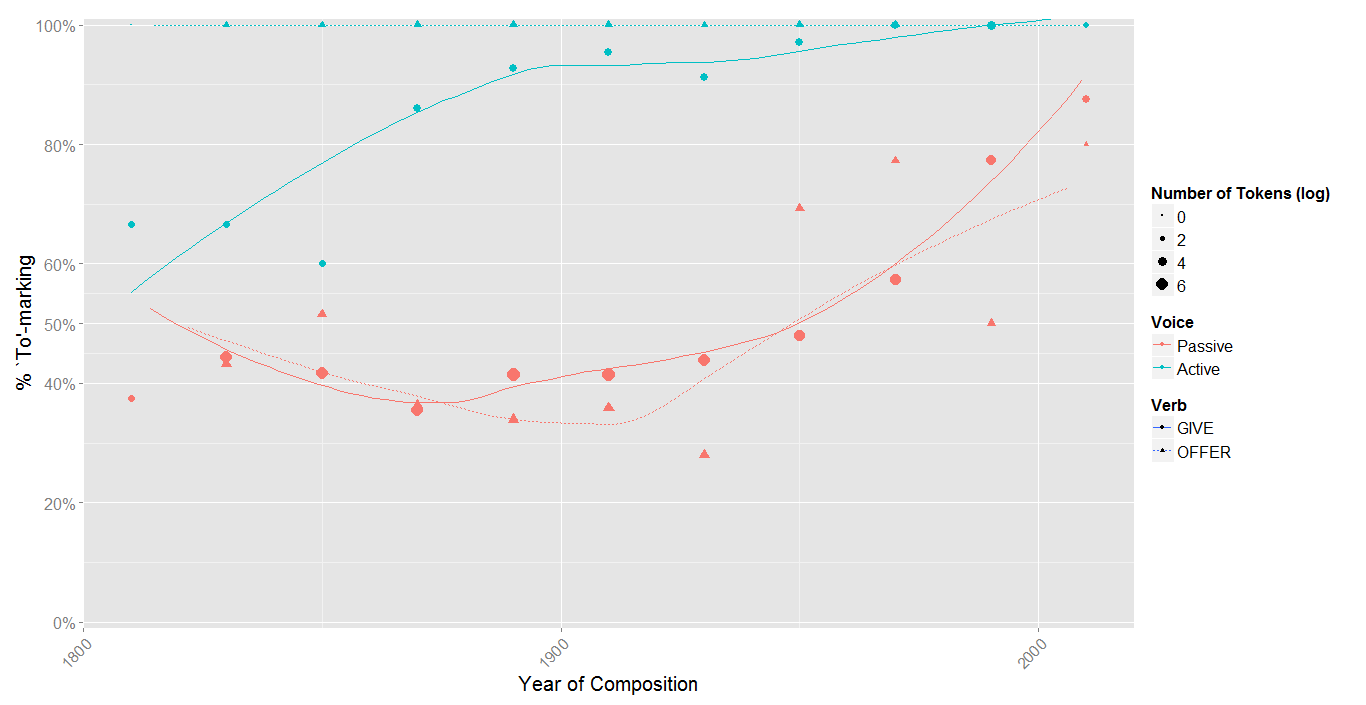
\includegraphics[width=\linewidth]{../images/recpro_to_am} 

}

\caption{LOESS lines for \textit{to} use in Modern American theme--recipient actives (with pronominal themes) and theme passives, both with pronominal recipients.\label{fig:amdata}}\label{fig:amtoset-graph}
\end{figure}

In combination with the results from Haddican's studies, this suggests that there is a complete dissociation between bare theme--recipients in the active and bare theme passives. All possible combinations of bare vs \textit{to}-marked theme--recipient actives and bare vs \textit{to}-marked theme passives are attested in different dialects/time periods. The analysis presented here predicts this dissociation, since the presence of case-based restrictions on locality are neither connected to nor solely dependent on pronoun cliticisation.

In order to investigate whether theme passives with bare recipients were restricted to theme pronouns, I extracted all tokens of theme passives with bare recipients after 1940 for a total of 337 tokens (with both full noun phrase and pronominal recipients. I coded all of the extracted tokens for the status of the theme: theme pronoun, theme noun, or theme empty (for empty categories, mostly subject relative clauses, or where information about the theme was unavailable). I found that theme nouns made up the largest number of tokens 63\%, with theme empty following at 24\%, and finally theme pronouns (almost exclusively \textit{it}) at 13\%. So, \textit{it} predominated among pronouns, probably because it is the most common theme pronoun. However, theme pronouns in general were the least likely to occur with bare recipients, probably because pronouns are rarer than full noun phrases in general in written text. The ample evidence for full noun phrase theme subjects with bare recipients reinforces the fact that bare recipients in active and passive clauses are unrelated.

\subsection{Swedish Verbs and Theme Passivisation}
As discussed above, Swedish presents one of the clearest cases for the P-incorporation analysis of dative-to-nominative conversion. In this subsection, I discuss data concerning claims that theme passivisation with bare recipients is also available with prefixed verbs. Since P-incorporation makes the recipient a valid target for subjecthood and blocks VP-internal scrambling, theme passivisation should generally be impossible in these cases, unless the recipient has moved. One type of potential counter-example that can be solved in this way are cases of purported theme passivisation with bare pronominal recipients. Cliticisation of pronominal recipients could explain why pronominal recipients can stay low in these cases.

\begin{exe}
	\ex Swedish:\label{ex:sw-offer-pass}
	\gll Ett nytt jobb erbjöds=honom.\\
A new job offered.PASS=him.OBL.\\
\trans `A new job was offered to him (\citealt{Anward.1989},\citealt{Falk.1990},\citealt{Lundquist.2006}).'
\end{exe}

If this is true, Swedish gives further clarity about the cliticisation process, since theme passivisation with unmarked recipients is \textbf{only} available with particle verbs. This suggests that in Swedish, the cliticisation process is restricted to DP pronouns. Pronouns in a dative PP (i.e., in non particle verbs) are unable to cliticise and thus serve as defective interveners for direct theme passivisation (see previous subsection).

\begin{exe}
	\ex Swedish:\label{ex:sw-give-pass}
	\gll *Ett äpple gavs honom.\\
	 An apple gave.PASS him.\\
	 \trans `An apple was given to him (\citealt{Anward.1989},\citealt{Lundquist.2006}).'
\end{exe}

However, \cite{Lundquist.2004} claims that there are examples of theme passivisation with full noun phrases with prefixed verbs.

\begin{exe}
	\ex Swedish:\label{ex:sw-offer-thepas}
	\gll Jobbet erbjöds mannen med den långa svarta kappan.\\
	job.DEF offered.PASS man.DEF with the long black coat\\
	'The job was offered to the man with the long black coat \citep[ex 26]{Lundquist.2004}.'
\end{exe}

If the prefixed verbs reflect P-incorporation, as I have argued, then direct theme passivisation is not a possible explanation (since the recipient is a valid target for subject movement). Instead, I claim that these are actually cases of recipient passivisation with theme topicalisation. Since Swedish is a V2 language, there is a strong ambiguity for sentence initial elements between a subject and topic interpretation. \cite{Lundquist.2004} provides examples in which themes are degraded when they occur in unambiguous subject positions (i.e., between an auxiliary and the passive participle).

\begin{exe}
	\ex Swedish:\label{ex:sw-relpass}
	\begin{xlist}
		\ex[ ]{\gll Mannen som erbjöds \textbf{jobbet} hade redan tackat ja till ett annat jobb.\\
		man.DEF who offered.PASS \textbf{job.DEF} had already thanked yes to a other job\\
		\trans `The man, who was offered the job, had already accepted another job \citep[ex. 51]{Lundquist.2004}.'}
		\ex[??]{\gll Mannen som \textbf{jobbet} erbjöds hade redan tackat ja till ett annat jobb.\\
		man.DEF who \textbf{job.DEF} offered.PASS had already thanked yes to a other job\\
		\trans `The man, to whom the job was offered, had already accepted another job \citep[ex. 52]{Lundquist.2004}.'}
	\end{xlist}
\end{exe}

Another piece of evidence comes from the distribution of recipient and theme passivisation in corpora. \cite{Lundquist.2004} shows that recipient passivisation is extremely prevalent in modern Swedish (with prefix verbs). This propensity is explained if purported examples of theme passivisation are actually cases of theme topicalisation, which is expected to happen at relatively low rates in a corpus.

One challenge for this view is that there are cases where the recipient seems to not (obligatorily) occur in subject position. Since Swedish generally requires expletives when the subject position is not filled, this analysis would require that null expletives be licensed in theme relative clauses. 

\begin{exe}
	\ex Swedish:\label{ex:sw-relpass2}
	\begin{xlist}
		\ex[ ]{\gll Jobbet som erbjöds \textbf{mannen} var mycket slitsamt.\\
		job.DEF which offered.PASS \textbf{man.DEF} was very tiring\\
		\trans `The job, which was offered to the man, was very tiring \citep[ex. 49]{Lundquist.2004}.'}
		\ex[ ]{\gll Jobbet som erbjöds \textbf{mannen} var mycket slitsamt.\\
		job.DEF which \textbf{man.DEF} offered.PASS was very tiring\\
		\trans `The job, which the man was offered, was very tiring \citep[ex. 50]{Lundquist.2004}.'}
	\end{xlist}
\end{exe}

Interestingly, \cite{Haddican.2015} notes that although theme passives with null recipients are generally judged unacceptable in American English, theme relative clauses are often judged much better. Since the relationship between theme relative clauses and bare recipients is replicated across at least two languages, it seems worthy of further research into the relationship between the head of relative clauses and the internal properties of the clause. However, such an investigation of relative clause structure is outside the scope of this dissertation.

\begin{exe}
	\ex Modern American English (Recipient Relatives):\label{ex:amen-relpass}
	\begin{xlist}
		\ex[ ]{The man, who was given the book, read.}
		\ex[?]{The man, who the book was given to, read.}
		\ex[??]{The man, who the book was given, read.}
	\end{xlist}
	\ex Modern American English (Theme Relatives):\label{ex:amen-rellpass2}
	\begin{xlist}
		\ex[?]{The book, which the man was given, was red}
		\ex[ ]{The book, which was given to the man, was red}
		\ex[??]{The book, which was given the man, was red}
	\end{xlist}
\end{exe}

\section{Conclusions}
This chapter analysed passivisation of recipient ditransitives. P-incorporation converted dative recipients into unmarked DPs, licensing dative-to-nominative conversion. This incorporation was seen on the surface in Dutch, German and Swedish. Oblique subjects were analysed by splitting the movement and case assignment properties of T into different searches (with different domains of application). In addition, surface theme passivisation with nominative themes were shown to arise from a number of possible mechanisms for avoiding locality violation, namely: relativised minimality, VP-internal scrambling, and recipient scrambling/cliticisation. Relativised minimality was argued to result in direct theme passivisation, where the theme moved to subject position directly from its base merged position.

%\bibliography{diss}

%\part{Conclusions and Further Implications}\label{part:form}
\chapter{Full Case Study in English Diachrony}
\section{Introduction}
This chapter applies the analysis presented in the previous three chapters to a large scale case study, namely diachronic development in recipient ditransitive syntax in the history of English. As discussed in the introduction, quantitative (and especially) diachronic studies can provide a useful independent verification of analyses developed on the basis of acceptability judgements. Crucially, data from language production can provide independent verification of theories developed primarily from language comprehension (i.e., acceptability judgements).

The problem of finding empirical validation of theoretical claims is made acute by the nature of the types of claims made in theoretical linguistics. Building on the work starting during the cognitive revolution in the 50s and 60s, the goal of generative linguistics has been to study the linguistic competence of speakers, which consists of the language specific information that is needed to use a language natively (CITATIONS). As will be shown below, this linguistic competence can be separated into grammatical and non-grammatical competences. Grammaticality reflects the ability of a grammar to associate a particular utterance with a particular meaning. However, given the rampant ambiguity in natural language, the grammar of natural languages often associates multiple utterances with a particular meaning (and multiple meanings with a particular utterance). An equally crucial aspect of being a native speaker of a language is knowing which of the options produced by the grammar to use in any particular circumstance. These choices are often impacted by language specific implementations of general social or psychological factors (CITATIONS). Unfortunately, it has been known since the beginning of this enterprise that there is no direct evidence of this knowledge (CITATION), which is typical of knowledge and psychological constructs. Instead, it has been necessary to deduce the nature of the linguistic knowledge by studying its effects on language performance (see CITATIONS-FROM-PHILLIPS-LAB for discussion of the fundamentally performative aspect of linguistic data).

One of the most prominent types of linguistic performance to be used in theoretical linguistics is the acceptability judgement. These judgements reflect a native speakers sensation of naturalness/unnaturalness upon encountering a particular linguistic utterance. These sensations have a cognitive reality similar to that of pain sensations (CITATIONS). A major advantage to the acceptability judgement is that even utterances that would never occur in natural production (due to the combination of factors each of which is extremely infrequent) can still be studied. However, as mentioned in the first chapter, grammaticality is only one aspect that contributes to the sensation of naturalness; other factors such as pragmatic concerns can often render a perfectly grammatical utterance unnatural (e.g., because there is a more concise grammatical way of conveying the same information). Trained linguists (and ideal native language informants) are able to minimise contextual factors that impact naturalness by attempting to evaluate the utterance in a number of hypothetical linguistic contexts, but these techniques cannot rescue a grammatical utterance that is ruled out because of universal, overwhelming problems. These non-grammatical problems often have a gradual impact on acceptability, reflect a gradient notion of pragmatic infelicity or psychological complexity (CITATIONS).

Quantitative studies of language performance is useful for isolating these gradient factors, so that they can be factored out when studying grammaticality using performance data. Since corpora (ideally) provide multiple instances of the relevant features in a variety of pragmatic contexts, the gradient effects of non-grammatical factors can be investigated for the observed contexts and statistically extrapolated to unobserved contexts. In addition, corpora provide a means of studying diachronic processes that cannot be studied using traditional acceptability judgements, since the earlier speakers in the diachronic process are unavailable for consultation. Assuming that language change cannot radically alter the underlying grammar (since the speakers of the new variety must participate in a speech community with speakers of the old variety), it is possible to provide independent evidence of the internal structure of the relevant grammatical processes.

This chapter will begin by reviewing the analyses from the previous three chapters and discussing the diachronic implication of these analyses. This will be followed by looking at three independent changes in the history of English. The first change is the change in recipient marking, ranging from synthetic dative case in Old English to the current distribution of `to' in modern American English. The second change reflects changes in the non-grammatical competence of speakers vis-a-vis active word orders in the history of English (i.e., when does the recipient occur before the theme and vis-a-versa). Finally, the fall and rise of recipient passivisation will be examined going from Old English to modern American English.

\section{Theoretical Issues}
	Since this dissertation argues that all languages have the same underlying configuration of recipient and theme (i.e., the recipient is introduced as a dative PP in the specifier of an applicative phrase), I predict that there should be no diachronic development in base generation. However, there are a number of transformations that can apply to the base generated order and different stages of the language can vary as to which operations are grammatical and when they should apply.
	One of the major factors that impact the surface realisation of recipients is allomorphy with respect to the morphological realisation of the dative P-head. The P-head itself can receive a null realisation or be spelled out overtly (e.g., as the preposition `to'). It can also trigger concord on its complement, which causes the realisation of synthetic dative case on elements in the noun phrase. As an instance of allomorphy, these variants can be sensitive to contextual information (e.g., the properties of surrounding elements). The nature of these links are the essence of Sassurian arbitrariness and are thus predicted to be subject to drift over centuries of language change.
	In addition to morphological variation, there are a number of syntactic operations that impact both the surface order of elements and their syntactic hierarchy. Since all of these operations are optional, any stage of the language could fail to have them. Thus, grammatical change is predicted to involve gaining or loosing one of the operations. These operations are one of the main sources of ambiguity that necessitates the non-grammatical component of language competence. Thus, change could also impact the rate at which these grammatical operations apply. VP-internal scrambling derives a theme--recipient order from the underlying recipient--theme order by moving the theme to a higher specifier of the applicative phrase. Cliticisation moves a pronominal element from being an independent syntactic head to being adjoined to a head in the verbal spine (here the head will always be little-v/voice). Finally, P-incorporation can move the dative P-head out of the PP and adjoin it to the next highest head. This renders the complement of the preposition a bare DP, which makes it eligible for receiving structural case.
	Looking at passivisation, the availability and probability of the transformations discussed in the previous chapter alters the availability of the theme and the recipient to raise to subject position and receive nominative case. In addition, languages vary as to the permissability of T in assigning subject properties. The main variation is in the treatment of PPs in the search for a subject. The assignment of nominative case (as a structural case) is restricted to DPs, a fact which does not vary diachronically (modulo the presence/absence of P-incorporation). However, the search for an argument to raise to subject position shows a variety of possible treatments for PPs. PPs can be valid targets for subject raising (oblique subjects), they can be invisible for subject raising (triggering direct theme passivisation), or they can be defective interveners (requiring one of the operations from the previous paragraph to create a non-intervening configuration).
	In the history of English, almost all of the changes discussed above occur. The realisation of dative P shifts from synthetic dative case to `to' alternating contextually with a null realisation. While VP-internal scrambling is grammatical in all stages of English, the conditioning factors change moving from Old English to modern American English. Cliticisation is lost during the history of American English, while P-incorporation becomes common place. Finally, all of the possible treatments of PPs in passivisation are attested (oblique subject, direct theme passivisation and defective intervention). Crucially, in every case of a change in grammaticality, the analyses presented here can account for the surface change by positing the gain/loss of a single syntactic operation.
\section{Recipient Marking}
Old English had synthetic dative case marking inherited from proto-Germanic. While there was a great deal of syncretism in the Old English case system \citep{AllAllen.1999}, there was a reliable distinction between accusative and dative case for many noun classes and in pronouns.

By the end of the Old English period (11th century), these distinctions were breaking down. Nominal case marking was no longer reliable. While both accusative and dative pronominal forms were still being used, the forms were no longer consistently distributed along the accusative/dative case distinctions (i.e., old dative case forms would be used where previously accusative case was required and vis-a-versa). Around this time, `to' began to be used for the first time to introduce recipients. In Old English, `to' had previously been restricted to goals and addressees, i.e., the indirect object of verbs of communication \citep{Allen.1999,McFadden.2002,OED.2013}. 

Throughout the Middle English period (i.e., up until about 1400), `to' became more prominent 

Changes in case marking
	- Loss of synthetic dative
	- `to' as realisation of dative P
	- Introduction of allomorphy and constant rate effects
	- The role of theme cliticisation
%\section{Active Order}
%	INSERT GRAPH OF ENGLISH WORD ORDERS
%	Throughout the history of English, both recipient--theme and theme--recipient orders have been possible. 
%	- No categorical change (or even tendency towards categorical change)
%	- Changes in sensitivity to pragmatic conditioning environments
%		- Sensitivity to weight in Early British English
%		- Sensitivity to animacy in American English
%	- Theoretical consequences
\section{Passivisation Order}
	Changes in passivisation of ditransitives is a more complex change. The situation in Old English is quite complex. \cite{Allen.1999} provides evidence that monotransitive datives are able to become oblique subjects in Old English, but she suggests that in ditransitives, putative oblique subjects are actually topics. To discuss this distinciton, she introduces the term ``fronted dative'', which is agnostic as to whether the fronted element is a topic or a subject. The argument about the status of fronted datives in ditransitive passives is made on the basis of Coordinate Subject Deletion facts.
	In Old English (as in Modern English), arguments are generally obligatory (i.e., neither subject nor object drop is licensed). However, when two sentences are coordinated and share the same subject, the subject does not need to be expressed in the second sentence (\ref{ex:OECSD}). In a corpus investigation, none of the fronted datives in ditransitive passives triggered Coordinate Subject Deletion, while a number of fronted nominatives did (see Table \ref{tab:AllenOECSD}). 

	\begin{table}
		INSERT ALLEN's CSD TABLE
		\label{tab:AllenOECSD}
	\end{table}

	\begin{exe}
		\ex \label{ex:OECSD} INSERT EXAMPLE OF OE CSD
	\end{exe}

	There are two problems with this argument. In the first case, the total number of coordinated passive sentences is not very large, so it is possible that the lack of dative examples is merely accidental. This is made even more serious because of Standard German facts. While Standard German is generally accepted to not have oblique subjects (CITATIONS), it does allow fronted dative elements to trigger coordinate topic deletion, but only if the two topic share the same case (CITATIONS). Assuming that Old English had the same rules, (a) Coordinate Subject Deletion would need to be distinguished from Coordinate Topic Deletion and (b) the fact that fronted dative elements are rarer than fronted nominative elements would need to be accounted for before any data was interpreted. 
	In additions to the problems with her argument discussed above, I have data from the Corpus of Old English Prose (CITATION) that suggests that fronted datives in Old English ditransitive passives were actually subjects. In Old English, the status of the theme and recipient as noun vs pronoun had a nearly categorical effect on active word order, with recipient pronouns coming before theme nouns and theme pronouns coming before recipient nouns and pronouns. The exact same ordering sensitivity is found for the fronted element in the passive, which can be explained if these fronted elements are subjects (oblique or otherwise) and the highest element in the active raises to subject in the passive. If they were topics, it is unclear why topicality should be sensitive to active word order in this way.

	INSERT TABLE HERE
	
	This match between active and passive orders ceases after the Old English period. The move from Old English to Modern English is characterised by the loss of recipient fronting. Much of this loss occurs during the 11th and 12th centuries (where our data is sparsest), however, by the 13th century, ditransitives with initial recipients are quite uncommon (see Fig. ). This loss of recipient fronting begins as a loss of oblique subjects. However, by at least 1375, dative--to--nominative conversion had become a live possibility \citep{Allen.1999}. Interestingly, this change in the origins of recipient subjects in passives (from oblique subjects to dative--to--nominative conversion) did not prevent (or seemingly alter) the loss of recipient passivisation.

	INCLUDE PROOF OF CONTINUITY

	INSERT FIGURE OF RECIPIENT PASSIVISATION

	Under the system proposed here, this change reflects a move away from having either PP passives or P-incorporation. Together these reflect a dispreference for manipulating PPs. If the PP cannot move to subject position or be incorporated, then theme passivisation becomes obligatory. While P-incorporation is grammatical (as can be seen by the existence of pseudo-passives and the occasional instance of dative--to--nominative conversion), it is strongly dispreferred, apparently because any such manipulation of PPs was dispreferred. This reflects a case where the grammar can generate possibilities that are selected against. In other words, for pseudo-passives P-incorporation is the only possible way of demoting the agent (assuming this is the main pragmatic role of passivisation). However, for ditransitives, P-incorporation is only one of a set of possible operations that license ditransitive passivisation. Building on previous generations loss of oblique subjects, there was a dispreference for manipulating PPs, which extended to the use of P-incorporation when other options were available.

	This separation of active and passive word orders continues in British English to the end of our data (in abt. 1911). However, the change is reversed in American English. Looking at data from the Corpus of Historical American English \citep{DavDavies.2010}, I extracted all instances of passive sentences involving the verbs `give' or `offer'. For `give', I hand coded all of the examples, while for offer I coded a sample of X tokens for each year. Each token was coded for the type of passive (theme, recipient, or monotransitive), the status of the recipient (full noun phrase or pronoun), and the marking of the recipient (presence/absence of `to'). For `offer', I also hand coded the status of the theme (full noun phrase or pronoun). For `give', I use a script to determine where the theme was (based on the type of passive coding) and then determined the status of the theme automatically.
	
	The result of this study shows that the main change in ditransitive passives in American English was an increase in the rate of recipient passivisation. In the early 19th century, there are essentially no examples of recipient passives. By the end of the 20th century, recipient passivisation rates match active word order rates (see Fig. X). Logistic regression models confirm that the change in recipient passivisation during this period is significant (INSERT STATS HERE). Just as in Old English, ditransitive passive word order reflected active ditransitive word order.

	INSERT TABLE COMPARING ACTIVE AND PASSIVE WORD ORDERS IN LATE 20th CENTURY AMERICAN ENGLISH

	According to the analyses proposed here, this change in American English reflects a normalisation of P-incorporation. In Early Modern English (and at least early 20th century British English), P-incorporation was a marked operation. If there was no other way of implementing passivisation (i.e., in the case of pseudo-passivisation), P-incorporation was available. However, if possible, speakers preferred to use other mechanisms for licensing passivisation. In American English, however, P-incorporation became a normal state of affairs. Given that the preposition is realised as $\emptyset$ in recipient--theme orders, there is no surface evidence against P-incorporation. Therefore, language learners only have indirect evidence for the rate of P-incorporation; this reliance on indirect evidence creates a situation that is ripe for language change.

\section{Conclusions}

\bibliography{diss}

\bibliographystyle{mcbride}
\bibliography{diss}
\end{document}
